\section{Schlussfolgerungen}
\label{sec:schlussfolgerungen}

In dieser Arbeit haben wir versucht Techniken und Methoden aufzuzeigen welche
es ermöglichen Entwicklungszyklen drastisch zu verkürzen. Ausgehend von einem
jährlichen Entwicklungszyklus wurden schrittweise Maßnahmen vorgestellt um die
Kadenz der Releases zunächst auf vierteljährlich, monatlich, wöchentlich und
zu guter Letzt auf täglich umzustellen. Dabei wurden nicht immer nur neue
Praktiken hinzugefügt sondern, sofern erforderlich auch bestehende als
schlecht aufgezeigt und für obsolet ja sogar hinderlich (Ballast) erklärt.
Eine Übersicht aller erwähnten Techniken und Methoden ist in
Tabelle~\ref{tab:uebersicht} auf Seite~\pageref{tab:uebersicht} aufgelistet. 

\begin{table}[htbp]
    \centering
        \caption{Übersicht über die Best Practices}
        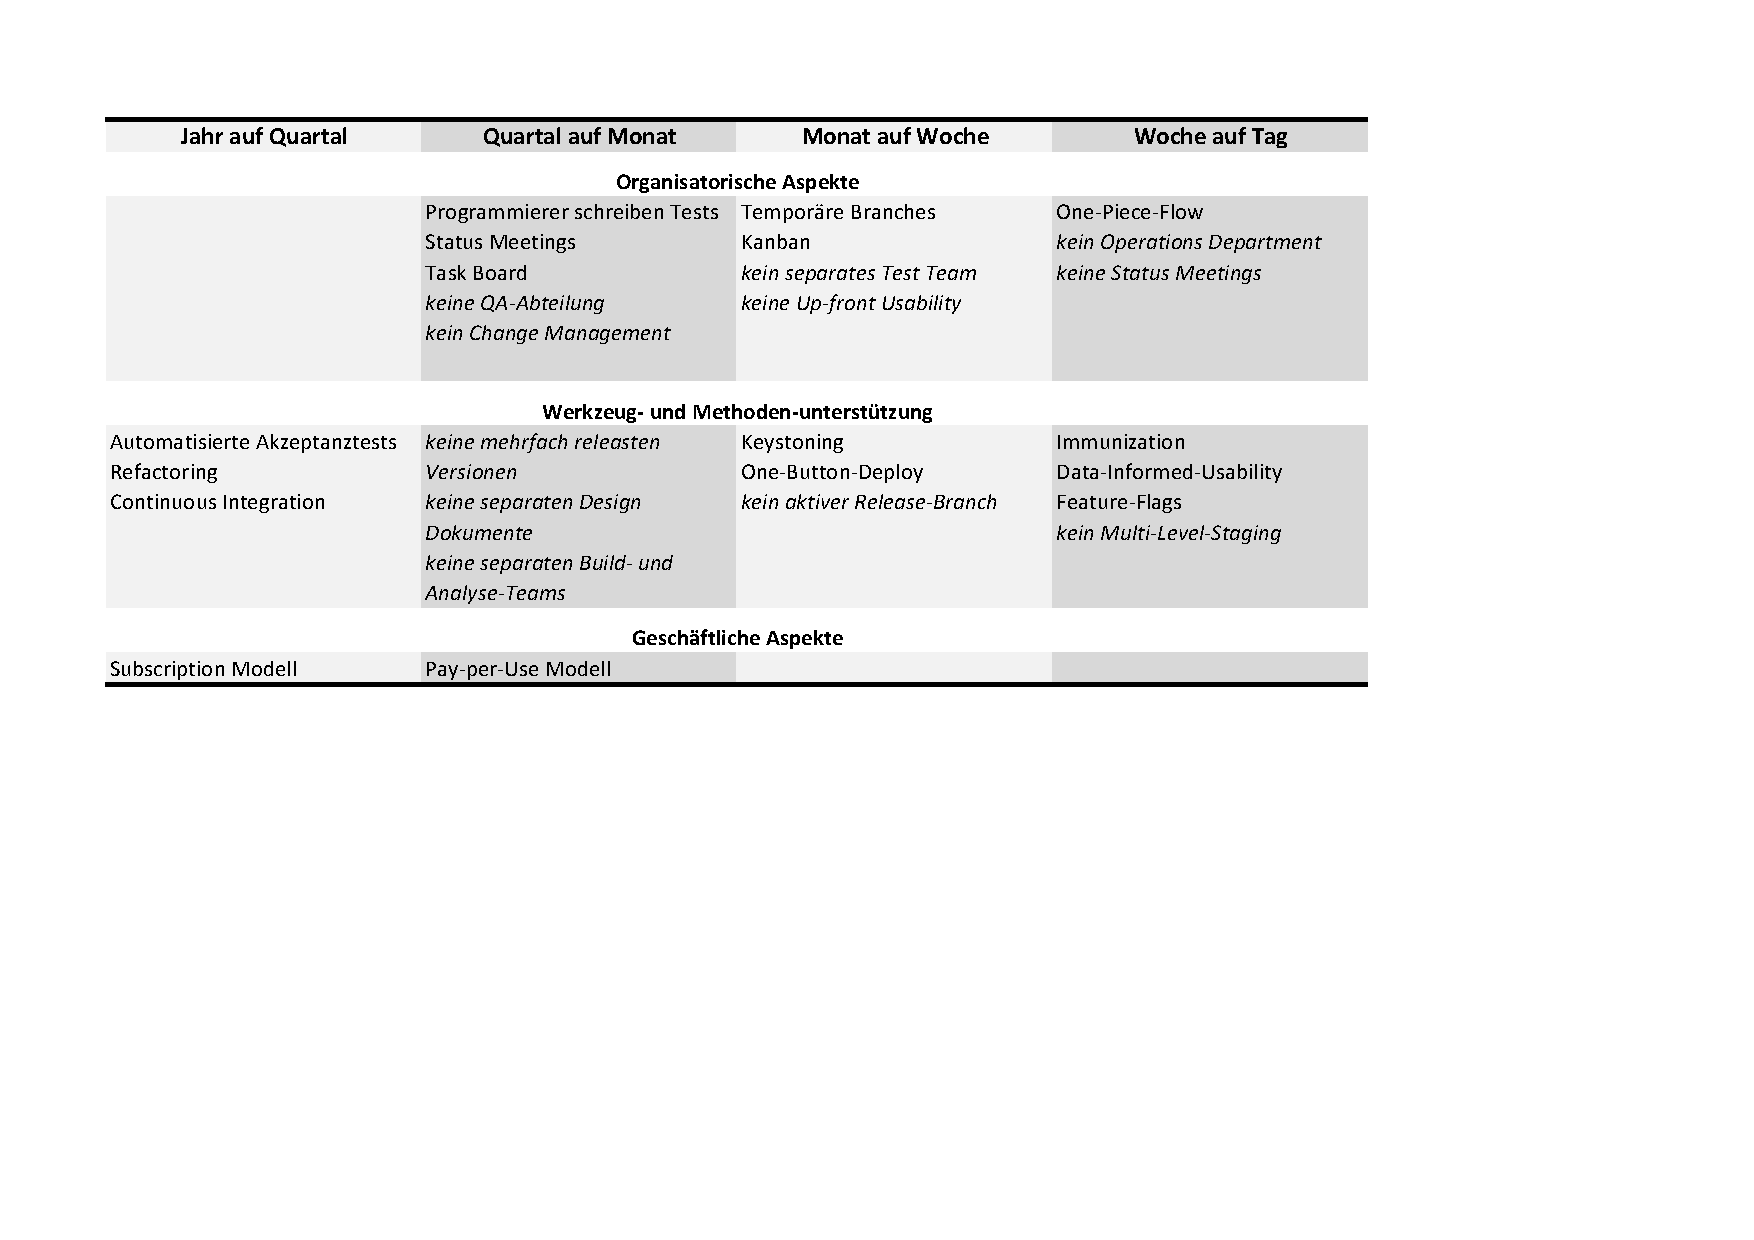
\includegraphics[trim = 50bp 265bp 185bp 56bp, clip, width=1.00\textwidth]{uebersicht}
    \label{tab:uebersicht}
\end{table}

In weiterer Folge wurden \emph{Success Stories} vorgestellt welche viele bzw.
Teile der in dieser Arbeit dargelegten Praktiken einsetzen, und damit
erfolgreich die Releasezyklen ihrer Software stark verkürzt haben. Die
Arbeitsabläufe der in den \emph{Success Stories} beschriebenen Firmen sind
dabei nicht selten inkrementell entstanden.

Zusammenfassend konnten laut den \emph{Success Stories} die folgenden Vorteile
gewonnen werden, wenn man es schafft seine Releasezyklen drastisch, bis hin
zum \emph{Continuous Deployment}, zu verkürzen:

\begin{itemize*}
    \item Fehler können rasch behoben werden da zwischen dem einspielen eines
          Fehlers und der Meldung über ein Problem nicht viel Zeit vergeht
    \item Regression wird sehr rasch erkannt
    \item Der Release einer neuen Version erzeugt keinen zusätzlichen Overhead
          (Releases werden sozusagen Non-Events) 
    \item Unmittelbares Feedback
    \item Feedback besteht aus sofort messbaren Kerndaten von echten Kunden
\end{itemize*}

Dass die vorgestellten Arbeitsweisen nicht perfekt sind wird von den
Betroffenen offen zugegeben. Die dabei erworbenen Vorteile überwiegen aber die
noch bestehenden Probleme. Siehe dazu auch das folgende Zitat von Andrew Bayer (Flickr):

\begin{quote}
\zitat{Does this mean we're never going to introduce bugs to our live site? Of
course not - but we're going to keep the number of bugs to hit the live site
to a minimum, and we've made it easy and fast to get bug fixes live as
well.}~\cite{digg4}
\end{quote}
